\chapter{Konwolucyjne sieci neuronowe}
\vspace{-1cm}
Konwolucyjna sieć neuronowa (CNN) jest specjalnym typem sieci, przystosowanej do analizy danych z obrazu \cite{baheti:cnnGuide, springer:cnnOverview}. Została zaprojektowana do automatycznego i adaptacyjnego uczenia się o przestrzennych wzorcach obecnych na obrazie oraz o hierarchii, jaką te wzorce tworzą. Rozpoznawanie wzorców przez sieć rozpoczyna się od najprostszych kształtów, a z każdą kolejną warstwą konstruowane są wzorce wyższego poziomu.

Tradycyjne sieci neuronowe były fatalnie przystosowane do analizy obrazów. Aby to zrozumieć, należy zobaczyć w jaki sposób obrazy są przechowywane w formie cyfrowej. Każdy obraz to macierz liczb rzeczywistych o wymiarach $\textbf{szerokość} \times \textbf{wysokość} \times \textbf{liczba kanałów}$. Z kolei standardowe sieci neuronowe oczekują na wejście danych w formacie tablicy jednowymiarowej. Problemem nie jest niezgodność reprezentacji danych, tylko fatalna skalowalność rozwiązania - w samej tylko warstwie wejściowej, sieć musi posiadać liczbę neuronów równą liczbie elementów w macierzy. Wraz ze wzrostem rozdzielczości analizowanych obrazów, lawinowo rośnie liczba parametrów sieci. Dla macierzy o wymiarach $200 \times 200 \times 3$ warstwa wejściowa musiałaby składać się z \textbf{120000 neuronów}, a w rzeczywistości wykorzystuje się obrazy o znacznie większych rozdzielczościach. Działanie na tak ogromnej liczbie parametrów jest kłopotliwe i znacznie utrudnia wytrenowanie sieci.

\section{Architektura}
W konwolucyjnych sieciach neuronowych obraz może być przetwarzany przy użyciu znacznie mniejszej liczby parametrów, ponieważ w danej chwili analizowany jest tylko jego fragment. Sieć neuronowa przechodzi po całym obrazie, skanując go fragment po fragmencie i wyszukując wzorce zakodowane w parametrach sieci. Parametry te podlegają zmianie w wyniku treningu sieci. Sieć konwolucyjna jest skonstruowana z kilku typów warstw:

\vspace{-0.5cm}
\begin{enumerate*}
\item \textbf{Warstw Konwolucyjnych} (z ang. \textit{Convolutional Layers}),
\item \textbf{Warstw ReLU},
\item \textbf{Warstw Łączeniowych} (z ang. \textit{Pooling Layers}),
\item \textbf{Warstw Normalizacyjnych} (z ang. \textit{Normalization Layers}),
\item \textbf{Warstw w Pełni Połączonych} (z ang. \textit{Fully-Connected Layers}).
\end{enumerate*}

\subsection{Warstwy Konwolucyjne}
Każda warstwa konwolucyjna składa się z tzw. \textbf{filtrów} (zwanych również \textbf{kernelami} lub \textbf{jądrami}). Każdy filtr jest macierzą o wymiarach niewielkich na szerokość i wysokość, ale w pełni obejmującej trzeci wymiar, czyli liczbę kanałów na piksel. Filtr jest przykładany po kolei do każdej możliwej pozycji na macierzy wejściowej i wykonywane są obliczenia, analogiczne do przykładu przedstawionego na rysunku \ref{ConvLayers}. \\

\begin{figure}[h]
\begin{center}
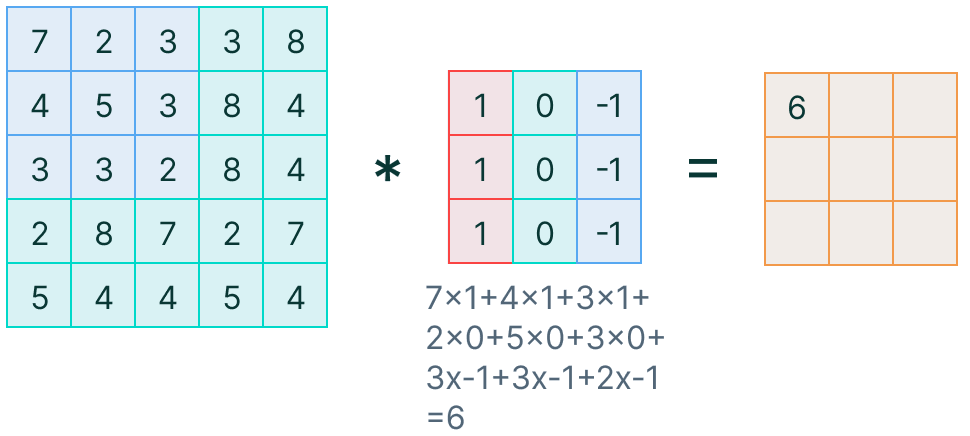
\includegraphics[width=15cm]{resources/figures/conv-layer.png}
\caption{Przykład działania filtru w warstwie konwolucyjnej}
\source{https://www.v7labs.com/blog/convolutional-neural-networks-guide}
\label{ConvLayers}
\end{center}
\end{figure}

\vspace{-0.5cm}
Parametry filtru (czyli elementy macierzy) definiują wzorzec przestrzenny, a ponieważ filtr jest przesuwany po całym obrazie, to zdefiniowany wzorzec może być wykryty w każdym miejscu obrazu. Wyniki zastosowania filtra zapisywane są do macierzy nazywanej \textbf{mapą cech} (z ang. \textit{feature map}). W każdej warstwie konwolucyjnej może być zdefiniowanych wiele filtrów, co oznacza że sieć uczy się wyszukiwać wiele wzorców na raz, niezależnie od siebie.

Warstwy konwolucyjne charakteryzują się kilkoma cechami:
\begin{enumerate*}
\item \textbf{Łącznością lokalną} (z ang. \textit{local connectivity}) - połączenia między neuronami występują tylko w obszarze definiowanym przez nakładane filtry.
\item \textbf{Uporządkowaniem przestrzennym} (z ang. \textit{spatial arrangement}) - ilość neuronów na wyjściu z warstwy, jak również sposób ich uporządkowania. Rozmiar wyjścia jest zdefiniowany poprzez trzy hiperparametry:
\begin{enumerate*}
\item \textbf{Głębokość} (z ang. \textit{depth}) - jest równa liczbie filtrów używanych w danej warstwie.
\item \textbf{Krok} (z ang. \textit{stride}) - oznacza liczbę pikseli, o jaką przeskakuje filtr po każdym dopasowaniu. Jeśli krok ma wartość 1, to filtr każdorazowo jest przesuwany tylko o jeden piksel. Im krok jest większy, tym mniejsze przestrzennie wolumeny będą produkowane.
\item \textbf{Wypełnienie zerami} (z ang. \textit{zero-padding}) - pozwala na kontrolę rozmiaru wolumenu wyjściowego poprzez dopełnienie zerami granic danych wejściowych.
\end{enumerate*}
\item \textbf{Udostępnianiem parametrów} (z ang. \textit{parameter sharing}) - ta sama macierz wag działa na wszystkie neurony w określonej mapie cech. To daje sieci możliwość rozpoznawania tych samych wzorców na różnych obrazach, nawet jeśli wzorce te są względem siebie przesunięte, obrócone lub przeskalowane o jakąś wartość. 
\end{enumerate*}

\subsection{Warstwy ReLU}
W tych warstwach wykorzystywana jest funkcja aktywacji ReLU \cite{brownlee:reluIntroduction}, której zadaniem jest podmiana wartości ujemnych na zero. To celowy zabieg, aby uniknąć ryzyka wyzerowania się sumowanych wartości.

\subsection{Warstwy Łączeniowe}
Są zwykle umieszczane pomiędzy dwoma warstwami konwolucyjnymi, aby zmniejszyć rozmiar przestrzenny mapy cech generowanej na wyjście z warstwy konwolucyjnej. Operują na każdym przekroju wolumenu wejściowego z osobna, zmniejszając jego rozmiar. Na sam koniec, pomniejszone przekroje są z powrotem układane w wolumen. Każda warstwa łączeniowa posiada dwa hiperparametry: \textbf{rozmiar okna} oraz \textbf{krok}. Wartości wyjściowe są obliczane według jednego z dwóch schematów - albo jest brane maksimum z wartości pokrytych oknem, albo też obliczana jest ich średnia.
Odpowiednio do wybranego schematu, warstwa łączeniowa jest typu \textit{Max Pooling} lub \textit{Average Pooling}.

Warstwa \textit{Max Pooling} wybiera największy element z każdego okna mapy cech, co skutkuje powstaniem mapy cech posiadającej najbardziej dominujące cechy poprzedniej mapy.

Warstwa \textit{Average Pooling} oblicza wartość średnią elementów należących do okna mapy cech, więc wynikiem działania jest mapa cech posiadająca uśrednione cechy oryginalnej mapy.

Na rysunku \ref{MaxPooling} zaprezentowano przykład działania warstwy łączeniowej typu \textit{Max Pooling}, gdzie rozmiar okna wynosi $2 \times 2$ i krok jest równy 2. Warstwy \textit{Max Pooling} są w praktyce częściej wykorzystywane, ponieważ dają większą skuteczność w uczeniu sieci.

\newpage
\begin{figure}[h]
\begin{center}
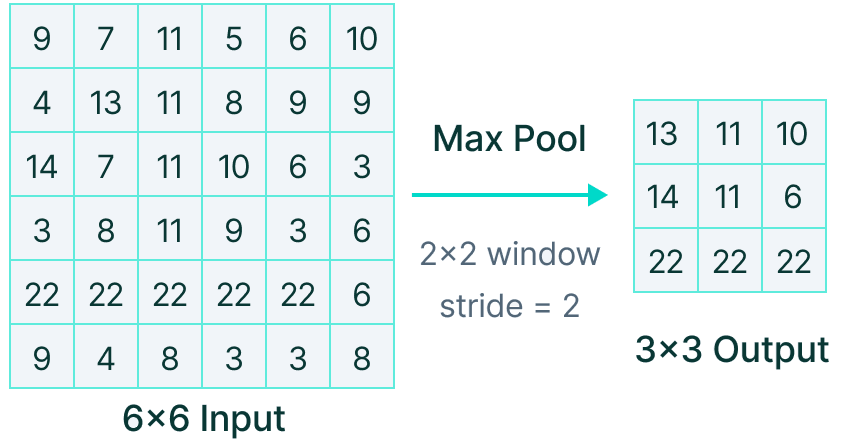
\includegraphics[width=15cm]{resources/figures/max-pool.png}
\caption{Przykład działania warstwy łączeniowej}
\source{https://www.v7labs.com/blog/convolutional-neural-networks-guide}
\label{MaxPooling}
\end{center}
\end{figure}

\vspace{-0.5cm}
\subsection{Warstwy Normalizacyjne}
Służą normalizacji wyjścia z warstw poprzednich. Warstwa normalizacyjna jest dodawana pomiędzy warstwą konwolucyjną a łączeniową, dzięki czemu każda z warstw może się uczyć niezależnie od siebie i w ten sposób uniknąć nadmiernego dopasowania modelu. Pomimo tych zalet, warstwy normalizacyjne są rzadko wykorzystywane w zaawansowanych architekturach, ponieważ mają niewielki wpływ na efektywność uczenia takich sieci.

\subsection{Warstwy w Pełni Połączone}
Stanowią ostatni etap w przepływie danych przez sieć konwolucyjną. Wygenerowane wcześniej mapy cech zostają przekształcone do postaci jednowymiarowej i wprowadzone na wejście do zwykłej, w pełni połączonej sieci neuronowej. Zadaniem tej sieci jest wygenerowanie ostatecznego wyniku zwracanego przez sieć.

\subsection{Funkcja aktywacji w ostatniej warstwie}
Ostatnia warstwa sieci konwolucyjnej ma zazwyczaj inną funkcję aktywacji, a jej wybór jest podyktowany typem zadania wykonywanego przez sieć neuronową. Z tego powodu najczęściej stosuje się funkcję:
\vspace{-0.3cm}
\begin{enumerate*}
\item \textbf{Softmax} \cite{wood:whatIsSoftmax} - dla klasyfikacji wieloklasowej;
\item \textbf{Sigmoidalną} \cite{saeed:sigmoidIntroduction} - dla klasyfikacji binarnej;
\item \textbf{Tożsamościową} - dla regresji do wartości ciągłych.
\end{enumerate*}

\subsection{Łączenie w całość}
Znając elementy składowe konwolucyjnej sieci neuronowej, przyjrzyjmy się jak one są ze sobą połączone. Z artykułu \cite{stanford:cnnCourse} dowiadujemy się, że najpopularniejszym schematem tworzenia sieci konwolucyjnej jest schemat następujący:

\noindent \texttt{INPUT -> ((CONV -> RELU) * N -> POOL?) * M -> (FC -> RELU) * K -> FC -> LAF}

\noindent gdzie:
\vspace{-0.5cm}
\begin{itemize*}
\item \texttt{INPUT} - warstwa wejściowa;
\item \texttt{CONV} - warstwa konwolucyjna;
\item \texttt{RELU} - warstwa ReLU;
\item \texttt{POOL?} - warstwa łączeniowa. Znak zapytania oznacza, że jest ona opcjonalna;
\item \texttt{FC} - warstwa w pełni połączona;
\item \texttt{LAF} - funkcja aktywacji warstwy ostatniej;
\item \texttt{N >= 0}, \texttt{M >= 0}, \texttt{K >= 0}.
\end{itemize*}

\section{Trening}
Trening sieci jest procesem poszukiwania odpowiednich filtrów dla warstw konwolucyjnych oraz odpowiednich wag dla warstw w pełni połączonych. Algorytm propagacji wstecznej \cite{kostadinov:backpropagation} jest powszechnie wykorzystywaną metodą nauki sieci neuronowej, gdzie funkcja straty \cite{brownlee:lossFun} oraz algorytm spadku gradientu \cite{kwiatkowski:gradientDescent} odgrywają kluczową rolę. Skuteczność sieci jest obliczana z funkcji straty przy propagacji wprzód dla danych ze zbioru treningowego, a parametry do wyuczenia (czyli filtry oraz wagi) są aktualizowane zgodnie z wynikami uzyskanymi przez funkcję straty, wspomagając się przy tym algorytmami propagacji wstecznej oraz spadku gradientu.

Przy nauce sieci neuronowych powszechnie korzysta się z dwóch funkcji straty: \textbf{entropii krzyżowej} (dla klasyfikacji wieloklasowej) \cite{brownlee:crossEntropy} oraz \textbf{błędu średniokwadratowego} (dla regresji do wartości ciągłych). Funkcja straty jest jednym z hiperparametrów sieci, który musi zostać wybrany przed rozpoczęciem treningu.

Aby trening sieci mógł się udać, należy zgromadzić odpowiednio duży oraz zróżnicowany zbiór danych. Następnie trzeba ten zbiór podzielić na 3 podzbiory:
\begin{enumerate*}
\item \textbf{Treningowy} - największy z podzbiorów. Jest używany przy treningu sieci, gdzie funkcja straty jest obliczana podczas propagacji wprzód i parametry sieci są aktualizowane podczas propagacji wstecznej.
\item \textbf{Walidacyjny} - wykorzystywany do nadzoru skuteczności sieci podczas trwania jej treningu oraz do dostrajania hiperparametrów sieci.
\item \textbf{Testowy} - powinien zostać użyty tylko jeden raz: po zakończeniu treningu sieci. Zbiór testowy służy ocenie skuteczności wytrenowanej sieci.
\end{enumerate*}

\begin{figure}[h]
\begin{center}
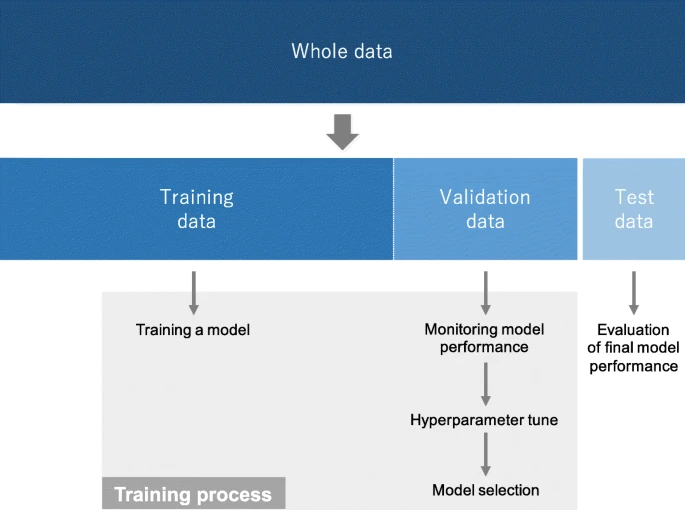
\includegraphics[width=15cm]{resources/figures/datasets.png}
\caption{Podział zbioru danych użytych do wyuczenia sieci}
\source{https://insightsimaging.springeropen.com/articles/10.1007/s13244-018-0639-9}
\label{DatasetDivision}
\end{center}
\end{figure}

Podział zbioru danych został zaprezentowany na rysunku \ref{DatasetDivision}. Oddzielne zestawy do walidacji i testów są konieczne, ponieważ zawsze istnieje potrzeba dostrojenia hiperparametrów sieci. Proces ten dokonuje się w oparciu o skuteczność sieci na zbiorze walidacyjnym, co sprawia że część danych z tego zbioru ,,wycieka'' do samego modelu. W rezultacie, sieć może osiągnąć efekt nadmiernego dopasowania się \cite{goyal:overfittingGuide} do zbioru walidacyjnego, mimo iż nie jest na nim uczona. Dlatego też do końcowej oceny skuteczności sieci stosuje się całkowicie osobny zbiór danych, który nie był wcześniej ,,widziany'' przez sieć neuronową. W ten sposób można zweryfikować poziom osiągniętej skuteczności na wytrenowanym modelu oraz sprawdzić, czy model ten nie został przeuczony na danych treningowych lub walidacyjnych.

\section{Przykłady z literatury}
Badając zagadnienie sieci konwolucyjnych, nie sposób nie wspomnieć o kilku wypracowanych modelach, które miały niebagatelny wkład w rozwój dziedziny:
\begin{enumerate*}
\item \textbf{LeNet} \\
Francuski naukowiec-informatyk Yann LeCun jest znany przede wszystkim ze swoich dokonań w zakresie optycznego rozpoznawania znaków oraz wizji komputerowej. W latach 90. XX wieku wraz ze swoimi współpracownikami zaprojektował wiele architektur, lecz największą sławę przyniosła mu sieć o nazwie LeNet. W obszernym artykule naukowym z 1998 roku \cite{lenet:article} została ona dokładnie przedstawiona i opisana. Sieć LeNet mogła być używana m.in. do rozpoznawania odręcznie napisanych cyfr oraz kodów pocztowych.
\item \textbf{AlexNet} \\
Była to pierwsza praca, która tak bardzo spopularyzowała wykorzystanie konwolucyjnych sieci neuronowych w wizji komputerowej. Stworzona przez trójkę naukowców z Uniwersytetu w Toronto i opisana w artykule \cite{alexnet:article}, AlexNet została wystawiona do konkursu \textit{ImageNet ILSVRC challenge} w 2012 roku i zdeklasowała swoich rywali, osiągając znacząco lepsze wyniki. Sieć miała architekturę podobną do LeNet, lecz była większa, głębsza i posiadała kilka warstw konwolucyjnych następujących bezpośrednio po sobie (w tamtych czasach normą było, aby po każdej warstwie konwolucyjnej następowała warstwa łączeniowa). AlexNet była tak ważnym kamieniem milowym, że jej nazwa pojawia się w każdej poważnej publikacji naukowej traktującej o historii rozwoju sieci konwolucyjnych.
\item \textbf{GoogLeNet} \\
Zwycięsca konkursu \textit{ILSVRC 2014}, stworzony przez zespół badawczy zdominowany przez pracowników firmy Google \cite{googlenet:article}. Jego najważniejszym wkładem w rozwój dziedziny było opracowanie tzw. \textbf{Modułu Incepcji} (z ang. \textit{Inception Module}), który pozwolił na radykalne zmniejszenie liczby parametrów sieci. Dla porównania, sieć GoogLeNet wystawiona do konkursu posiadała ,,zaledwie'' 4 miliony parametrów, podczas gdy AlexNet miała ich aż 60 milionów. Co więcej, GoogLeNet zastąpił większość warstw w pełni połączonych warstwami łączeniowymi typu \textit{Average Pooling}, co pozwoliło na pozbycie się parametrów mających niewielki wpływ na zachowanie sieci. Istnieje kilka wersji sieci GoogLeNet, najpopularniejszą z nich jest \textbf{Inception-v4}.
\item \textbf{VGGNet} \\
Stworzona przez Karen Simonyan i Andrew Zissermana, wykazała że odpowiednia głębokość jest kluczowym elementem dobrego zachowania sieci \cite{vggNet:article}. Najlepsza sieć VGGNet posiada 16 warstw i charakteryzuje się jednorodną architekturą, w której od początku do końca wykorzystywane są tylko konwolucje o wymiarach $3 \times 3$ oraz łączenia o wymiarach $2 \times 2$.  Największą wadą sieci jest jej ogromna liczba parametrów - dla wersji z 16 warstwami było to 140 milionów. Większość parametrów jest w warstwach w pełni połączonych, lecz badacze po pewnym czasie odkryli że warstwy te mogą zostać usunięte bez znacznej szkody dla skuteczności sieci.
\item \textbf{ResNet} \\
Zwycięsca konkursu \textit{ILSVRC} w 2015 roku, opracowany przez grupę badawczą z firmy Microsoft \cite{resnet:article}. Wyjątkowość tej architektury polega na wprowadzonych innowacjach, dzięki którym stał się możliwy trening sieci o znacznie większej liczbie warstw ukrytych. Było to ważne wydarzenie, ponieważ otworzyło zupełnie nowe możliwości przed badaczami. Przed opublikowaniem sieci ResNet, konwolucyjne sieci neuronowe zdawały się być nie do wytrenowania przy więcej niż kilkunastu warstwach ukrytych. Powodem takie stanu rzeczy było występowanie zjawiska \textbf{zaniku i eksplozji gradientu} \cite{bohra:vanishingGradient}, z którym naukowcy próbowali walczyć, lecz nieskutecznie. Dopiero twórcy architektury ResNet znaleźli odpowiedź na rozwiązanie tego problemu.
\end{enumerate*}

\section{Obszary zastosowań}
Konwolucyjne sieci neuronowe są obecnie wykorzystywane z sukcesem w wielu zadaniach z zakresu wizji komputerowej \cite{kumar:cnnApplications}. Wśród nich można wymienić:
\begin{enumerate*}
\item \textbf{Rozpoznawanie twarzy} - sieci konwolucyjne są powszechnie używane do wykrywania twarzy na obrazach. Sieć może wykrywać i rozpoznawać z dużą dokładnością różne cechy twarzy, takie jak oczy, nos i usta, redukując przy tym zniekształcenia powstałe na skutek złego oświetlenia obrazu.
\item \textbf{Rozpoznawanie emocji} - sieci konwolucyjne okazały się bardzo dobrze sprawdzać przy klasyfikacji różnych wyrazów twarzy, odzwierciedlających emocje człowieka. Sieciom w klasyfikacji nie przeszkadza zmienna pozycja twarzy wobec kamery oraz zmienne warunki oświetleniowe.
\item \textbf{Wykrywanie obiektów} - odbywa się poprzez klasyfikację obiektów na podstawie ich kształtu, kolorów oraz innych cech charakterystycznych dla danej grupy obiektów. Odpowiednio wytrenowana sieć konwolucyjna potrafi wykrywać bardzo szeroką gamę obiektów. Do wykrywania obiektów wykorzystuje się techniki segmentacji semantycznej oraz instancyjnej.
\item \textbf{Samochody autonomiczne} - sieci konwolucyjne są stosowane jako podstawowy komponent oprogramowania modelu percepcji opartego na obrazie z kamer. Trening sieci odbywa się przy wykorzystaniu techniki zwanej \textit{uczeniem ze wzmocnieniem}, która koncentruje się na pozytywnych i negatywnych informacjach zwrotnych ze środowiska, aby poprawić zachowanie sieci w danych sytuacjach.
\item \textbf{Tłumaczenie automatyczne} - okazuje się, że sieci konwolucyjne po odpowiednim treningu znakomicie sobie radzą z automatycznym tłumaczeniem, a przetłumaczone teksty charakteryzują się wysokim poziomem zgodności z oryginałem.
\item \textbf{Analiza danych medycznych} - modele uczenia maszynowego znalazły szerokie pole zastosowań w branży medycznej. Konwolucyjne sieci neuronowe mogą być użyte np. do identyfikacji guzów oraz innych nieprawidłowości na obrazach rentgenowskich. Są również stosowane przy wykrywaniu nowotworów na obrazach z badania tomografii komputerowej. Wytrenowana sieć jest w stanie wykrywać raka z dużą skutecznością, dochodzącą do 95\%. Dla porównania, lekarze-patolodzy biorący udział w badaniach osiągali skuteczność poniżej 90\%.
\item \textbf{Uwierzytelnianie biometryczne} - biometryczne uwierzytelnianie tożsamości użytkownika odbywa się na podstawie identyfikacji zestawu cech fizycznych, związanych z daną osobą. Sieci konwolucyjne świetnie się do tego sprawdzają. 
\item \textbf{Klasyfikacja dokumentów} - sieci konwolucyjne mogą klasyfikować dokumenty do różnych kategorii. Kategoria może być identyfikowana na podstawie treści dokumentu, rozkładu tekstu lub wielu innych cech. Konwolucyjne sieci neuronowe dla lepszego zrozumienia dokumentu mogą analizować zarówno tekst, jak i obraz. Modele CNN są również z powodzeniem stosowane do generowania streszczeń i podsumowań dokumentów na podstawie ich zawartości.
\item \textbf{Segmentacja trójwymiarowych danych medycznych} - konwolucyjne sieci neuronowe znalazły swoje zastosowanie także w segmentacji skanów obrazowania medycznego, takich jak obrazy z badania tomografii komputerowej lub rezonansu magnetycznego. Wytrenowana sieć konwolucyjna potrafi pobrać wycinek obrazu ze skanu 3D i określić, gdzie w obrębie tego obrazu znajdują się poszczególne rodzaje tkanek, a także konkretne narządy człowieka.
\end{enumerate*}

\section{Problemy i wyzwania na przyszłość}
Przed naukowcami pracującymi nad rozwojem sieci konwolucyjnych stoi szereg trudnych wyzwań, z którymi będą zmuszeni się zmierzyć.

\subsection{Wykorzystanie pamięci}
Jednym z najwęższych gardeł do rozważenia przy projektowaniu sieci konwolucyjnych jest ilość oraz rodzaj dostępnej pamięci, oferowanej przez współczesne karty graficzne. Większość kart jest ograniczona rozmiarem pamięci nieprzekraczającym kilku gigabajtów, co może być niewystarczające dla bardzo głębokich sieci konwolucyjnych z ogromną liczbą parametrów. Ponadto na sieci konwolucyjne mogą zostać nałożone restrykcyjne wymogi maksymalnego czasu odpowiedzi, co oznacza że wydajność sprzętu na którym sieci są uruchomione nagle zyskuje na znaczeniu. Więcej rozważań na temat efektywnego wykorzystania pamięci przez konwolucyjne sieci neuronowe można znaleźć w artykule \cite{cnn:memoryRequirements}.

\subsection{Zagrożenia bezpieczeństwa}
Sieci konwolucyjne są obecnie szeroko wykorzystywanym rozwiązaniem, począwszy od edytorów zdjęć i wideo, a skończywszy na oprogramowaniu medycznym i samochodach autonomicznych. Chociaż te sieci niesamowicie zbliżyły się w ostatnich latach do postrzegania świata w sposób zarezerwowany dotychczas tylko zwierzętom i ludziom, to wciąż istnieje wiele sytuacji w których sieć neuronowa całkowicie traci swoją skuteczność i generuje błędne wyniki. Głównym źródłem takich problemów są cyberataki dokonywane przez hakerów, a lwią część ataków stanowią tzw. \textbf{ataki kontradyktoryjne} (z ang. \textit{adversarial attacks}) \cite{dickson:adversarialMl}. Ataki te polegają w skrócie na dokładaniu do obrazu szumów niewidocznych dla człowieka, które wprowadzają sieć neuronową w błąd. Badania prowadzone w tej dziedzinie przyniosły już wiele zaskakujących wyników. Przykładowo, naukowcy z grupy badawczej LabSix w 2017 roku opublikowali artykuł \cite{labsix:foolingNNs}, w którym pokazali że odpowiednio zmodyfikowana zabawka w kształcie żółwia potrafi całkowicie zmylić popularną sieć neuronową klasyfikującą obrazy, czyli \textit{Google Inception-v3}. Modyfikacje są niezauważalne dla człowieka, a polegały na wprowadzeniu szumów do malowania pokrywającego żółwia. W efekcie, niezależnie od kąta ustawienia żółwia, sieć neuronowa będzie uparcie klasyfikować go jako karabin. Rysunek \ref{TurtleAdversarialAttack} przedstawia stopklatkę z filmu zawartego w opublikowanym artykule.

Bardziej niebezpiecznym przykładem niecnego wykorzystania ataków kontradyktoryjnych są manipulacje przy znakach drogowych, które mają wprowadzać samochody autonomiczne w błąd. Jak wykazały wyniki badań opublikowane w artykule \cite{adversarial:roadSignAttacks}, wystarczy nakleić kilka niepozornych nalepek na znak STOP, aby system rozpoznawania znaków drogowych zaczął go klasyfikować inaczej, np. jako znak ograniczenia prędkości. Testy zostały przeprowadzone na systemie wytrenowanym przez autorów badania, a nie na jakimś komercyjnie dostępnym modelu samochodu autonomicznego, dlatego można założyć że te konkretne ataki nie zadziałałyby na systemy zamontowane w samochodach Tesli lub Waymo. Niemniej jednak, ponieważ algorytmy na których opierają się systemy komercyjne nie różnią się zbytnio w swej zasadzie działania (mogą być co najwyżej inaczej wytrenowane), dlatego należy przyjąć że tego typu ataki są wciąż jak najbardziej możliwe. \\

\begin{figure}[h]
\begin{center}
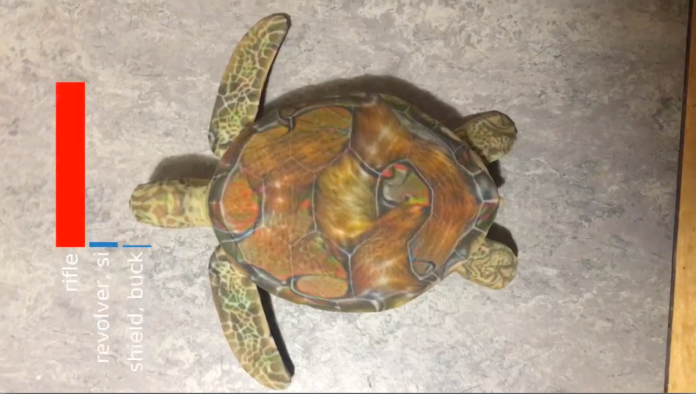
\includegraphics[width=15cm]{resources/figures/ai-adversarial-attack-turtle.png}
\caption{Przykład ataku kontradyktoryjnego - żółw klasyfikowany jako karabin}
\source{https://www.labsix.org/physical-objects-that-fool-neural-nets}
\label{TurtleAdversarialAttack}
\end{center}
\end{figure}

\vspace{-0.5cm}
Pewną iskierką nadziei na rozwiązanie tego palącego problemu są badania naukowców z MIT oraz laboratorium MIT-IBM Watson \cite{cnns:neuroscienceProtection}, gdzie badacze przedstawiają nową architekturę o nazwie VOneNet, opartą o połączenie aktualnych technik głębokiego uczenia maszynowego z aktualnym stanem wiedzy na temat neurobiologii. Uzyskana w ten sposób architektura wykazuje większą odporność na ataki kontradyktoryjne oraz charakteryzuje się bardziej przewidywalnym zachowaniem.

\subsection{Klasyfikacja obiektów z przekształceniami}
Jednym z wielu wyzwań w dziedzinie wizji komputerowej jest radzenie sobie ze zmiennością danych występujących w świecie rzeczywistym. Ludzki narząd wzroku potrafi prawidłowo rozpoznać obiekt na obrazie, nawet jeśli:
\vspace{-0.5cm}
\begin{itemize*}
\item obiekt sfotografowany jest pod różnymi kątami;
\item obiekt jest przedstawiony na różnych tłach;
\item zdjęcie zostało zrobione w różnych warunkach oświetleniowych.
\end{itemize*}

\begin{figure}[h]
\begin{center}
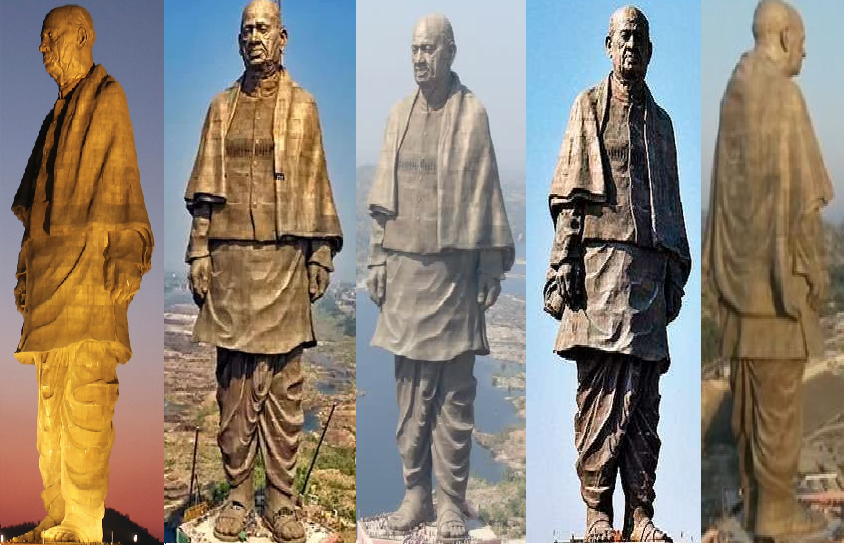
\includegraphics[width=15cm]{resources/figures/object_with_transitions.png}
\caption{Ta sama rzeźba na pięciu różnych ujęciach.}
\source{https://iq.opengenus.org/disadvantages-of-cnn}
\label{SculptPhotos}
\end{center}
\end{figure}

\vspace*{-1.5cm}
Gdy obiekty są częściowo zakryte lub nietypowo oświetlone, ludzki wzrok wciąż jest w stanie znaleźć informacje potrzebne do prawidłowej klasyfikacji obiektu na obrazie. Jednak stworzenie konwolucyjnej sieci neuronowej o takich właściwościach jest zadaniem bardzo trudnym, o czym przekonało się wielu badaczy. Sama pozycja obiektu na fotografii nie stanowi większego problemu, ale jeśli obiekt jest fotografowany pod różnymi ujęciami (jak to ma miejsce na rysunku \ref{SculptPhotos}), wtedy wiele popularnych modeli sieci konwolucyjnej będzie miało ogromny problem z prawidłowym rozpoznaniem obiektu. Rozwiązaniem tego problemu może być rozszerzenie zbioru danych treningowych o fotografie z odpowiednimi przekształceniami obiektu, o ile zostanie to zrobione w sposób umiejętny. Nie zawsze jednak jest to możliwe, dlatego też potrzeba dalszych badań nad sposobami obsłużenia tego problemu.

\section{Podsumowanie}
Sieci konwolucyjne to niezwykle obszerny i zarazem fascynujący temat, którego dokładne omówienie wykracza poza zakres tej pracy. W niniejszym rozdziale zostały poruszone tylko te wątki, które według autora były kluczowe do zrozumienia podstawowych elementów zagadnienia. W celu dalszego pogłębienia wiedzy zaleca się samodzielną eksplorację tematu, a dobrym punktem wyjścia może być literatura cytowana w tym rozdziale.